% !TEX TS-program = xelatex
% !TEX encoding = UTF-8 Unicode


% TODO: ik heb een goed idee waar het naar toe moet hoor, tis gewoon de uitvoering en flow dat moet kloppen. Ik ben van plan het eerst eens uit te werken voor een bepaald onderdeel van het literatuur hoofdstuk, te reviewen met jou en dan die stijl\flow\template toepassen voor de andere secties in dat hoofdstuk

\providecommand{\home}{../..}
\documentclass[\home/main.tex]{subfiles}

\begin{document}

\chapter{Background and review of related work} \label{ch:lit}

The goal of the following chapter is to provide the preliminaries and a review of relevant work in the field of robotic manipulation of deformable objects. To provide some historical context, we first discuss how \emph{standard robotic manipulation pipelines} can be used for manipulating deformable objects in Section~\ref{sec:lit_traditional}. Next, in Section~\ref{sec:lit_learning} we introduce how the inherent limitations of engineered motor control architectures can be overcome by using \emph{learning-based methods}. We break this section down into subsections introducing supervised learning, deep neural networks and reinforcement learning. This is followed by surveying their applications in recent robotic manipulation work. Given the general property that learning-based methods are data-hungry, we continue this discussion by reviewing the role of \emph{large datasets} for robotic learning in Section~\ref{sec:lit_datasets}. An alternative approach to generating data is to use synthetic data. To this end, we discuss the role of \emph{simulation} and the corresponding transferability problems in Section~\ref{sec:lit_simulation}. Critical to robotic learning of manipulation skills is some metric of task success, generally labelled as reward function. The role and methods to obtain \emph{reward functions} for robotic learning, and deformable objects manipulation in particular, is reviewed in Section~\ref{sec:lit_reward_learning}. Finally, we discuss the idea and corresponding literature of \emph{instrumenting the process with sensors} to facilitate the learning process in the manipulation environment in Section~\ref{sec:lit_instrumentation}.

\section{Manipulating deformable objects} \label{sec:lit_traditional}

This section provides important historical context and prior work in the rigid and deformable object manipulation literature. First, we discuss the traditional control approach to rigid object manipulation for robots and how these methods are challenging to generalize towards deformable object manipulation. Next, we provide a definition and categorization of deformable objects. For each category, we provide common tasks and solutions identified in literature.

\subsection{Manipulating rigid objects}
Grasping and manipulation problems in robotics are traditionally solved by manually engineering subsystems for perception, planning and control \autocite{Siciliano2008}. A popular approach is using images as input observation to control the robot's motions. This approach is motivated by the advantage that images enable closed-loop control: non-contact and real-time measurements of the environment can be used to provide feedback to the motion trajectory of the robot. This principle is generally known as visual servoing \autocite{Hutchinson1996} and was first introduced in~\citeyear{Hill1979} by \textcite{Hill1979}. An archetypical pipeline consists of the following steps to grasp and manipulate an object \autocite{Corke1996}. First, observations such as images are used to estimate the state of the object. This state estimation stage usually executes pixel manipulations and image filtering in order to extract features. This object state is used to interpret the scene to calculate the relative position of the target object from the robot end-effector. Once the object is identified, it can be modelled to identify a suitable grasping point. Next, these grasping points are given to a motion planning system that calculates a trajectory to move the end-effector to the desired position and orientation. Finally, a low-level controller sends motor commands to the actuators to move the robot. An example of this archetype control pipeline is displayed in \cref{fig:canonical_robotic_manipulation_engineered_pipeline}.

\begin{figure}[p]
    \centering
    \subfile{figures/canonical-robotic-manipulation-pipeline/fig-canonical-robotic-manipulation-pipeline.tex}
    \vspace*{-10mm}
    \caption[Canonical engineered manipulation pipeline.]{\textbf{Canonical engineered manipulation pipeline with examples of each module.} Cameras record observations that are used to estimate the state of the cloth downstream. The modelling module calculates the deformations on the cloth if certain manipulations are executed. A planning module calculates the desired end-effector trajectory and sends the corresponding joint position to a low-level controller.
    }
    \label{fig:canonical_robotic_manipulation_engineered_pipeline}
\end{figure}

% Probleem met traditionele pipelines toepassen voor vervormbare objecten
Engineering modular, hand-tuned motor control pipelines have been successful for applications in manufacturing \autocite{Clocksin1985,Mochizuki1987}, car steering \autocite{Dickmanns1988}, robotic ping-pong \autocite{Andersson1987}, juggling \autocite{Rizzi1993} as well as fruit picking \autocite{Harrell1989}. However, all of these applications operate under the condition of rigid objects: the shape of the object will not change on contact.
When manipulating objects, this is of importance for determining stable grasping points. More concretely, restraining rigid objects relies on \textit{form closure} \autocite{Nguyen1988} or \textit{force closure} \autocite{Bicchi1995}: fully constraining relative motion of the object or having contact points that can counteract an external wrench through friction.
However, in the case of deformable objects, the object can deform during grasping and manipulation. This leads to exponentially higher dimensional configuration spaces compared to rigid object manipulation \autocite{Foresti2004}. For example, achieving form closure becomes impossible as it requires immobilizing every degree of freedom. Similarly, force closure becomes computationally intractable as it requires constantly incorporating the adapted shape of the object. For example, we visually show (\cref{fig:force_closure_deform_object}) the deformations that occur when grasping a plastic cup versus a rigid glass when trying to achieve force closure. Furthermore, manipulation requires reasoning about the target shape of the object. These properties make many rigid object manipulation techniques hard to extend in the deformable object domain. Unfortunately, to date, the vast majority of robotic manipulation work deals with rigid objects whereas many objects are of deformable nature \autocite{Siciliano2008}.

\begin{figure}[htbp]
    \centering

    \begin{subfigure}[b]{0.95\textwidth}
        \centering
        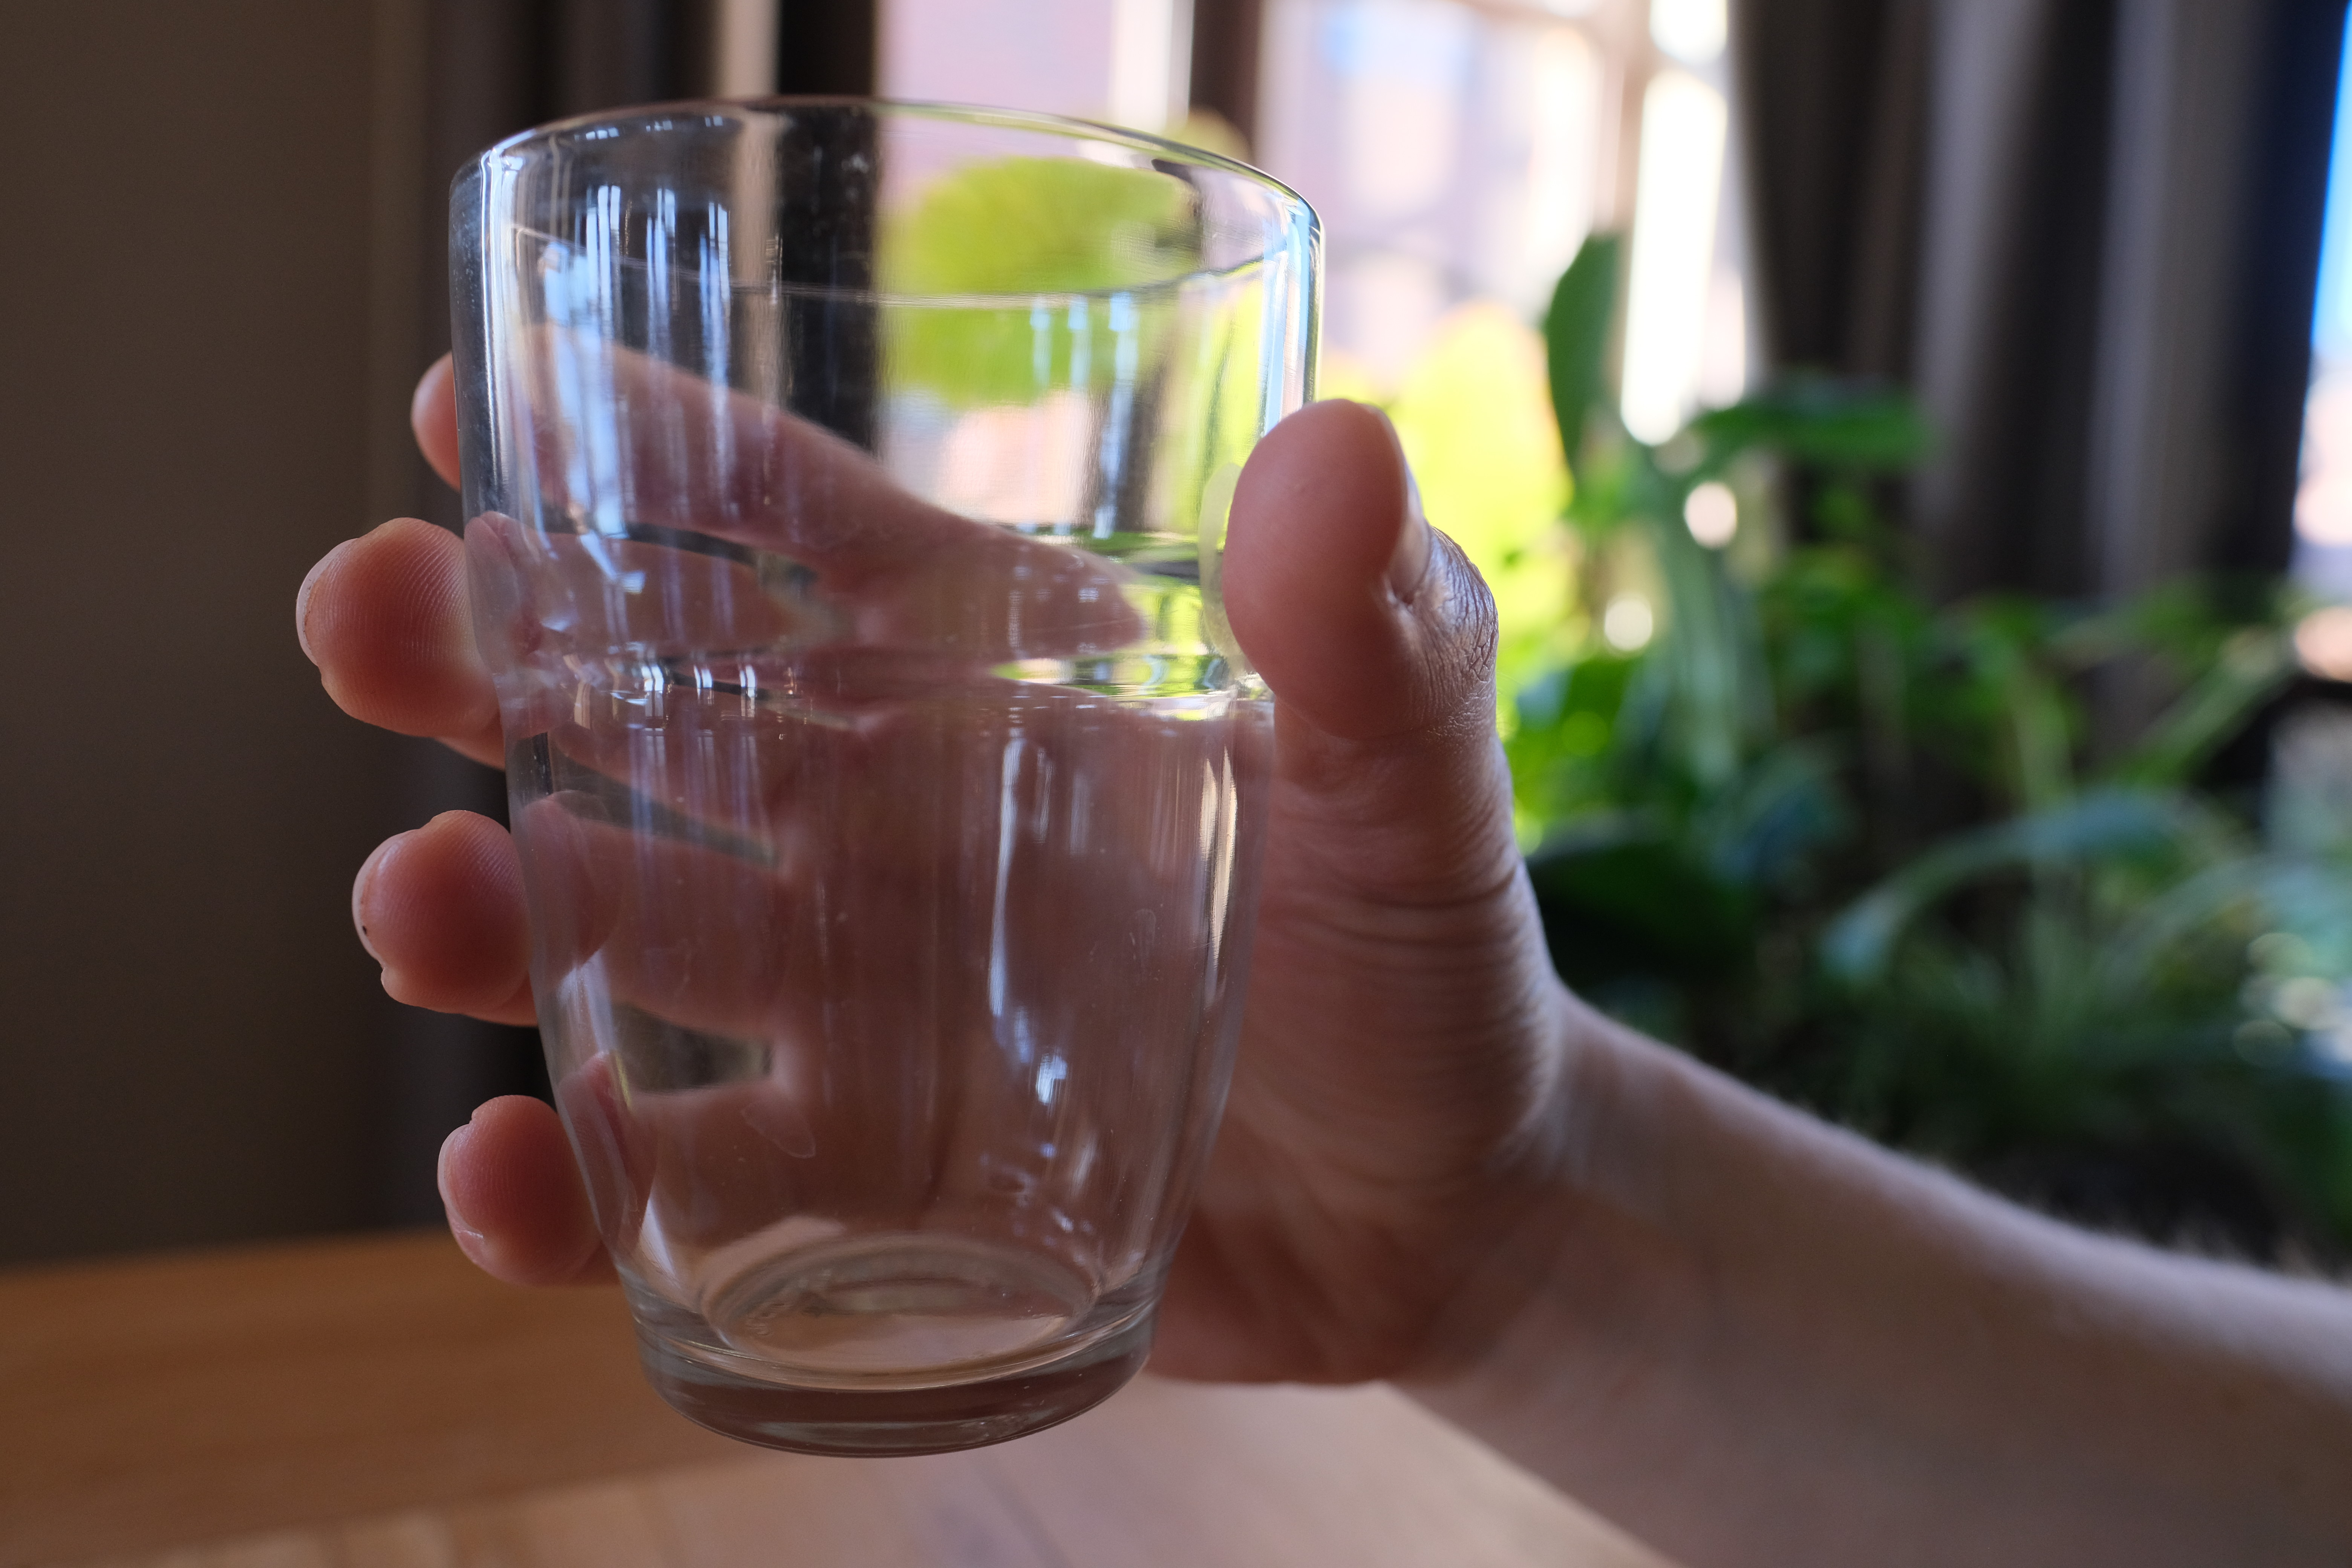
\includegraphics[keepaspectratio, width=\textwidth]{figures/fig_glass.jpg}
        \caption{}
        \label{fig:force_closure_deform_object_glass}
    \end{subfigure}
    \par\medskip
    \begin{subfigure}[b]{0.95\textwidth}
        \centering
        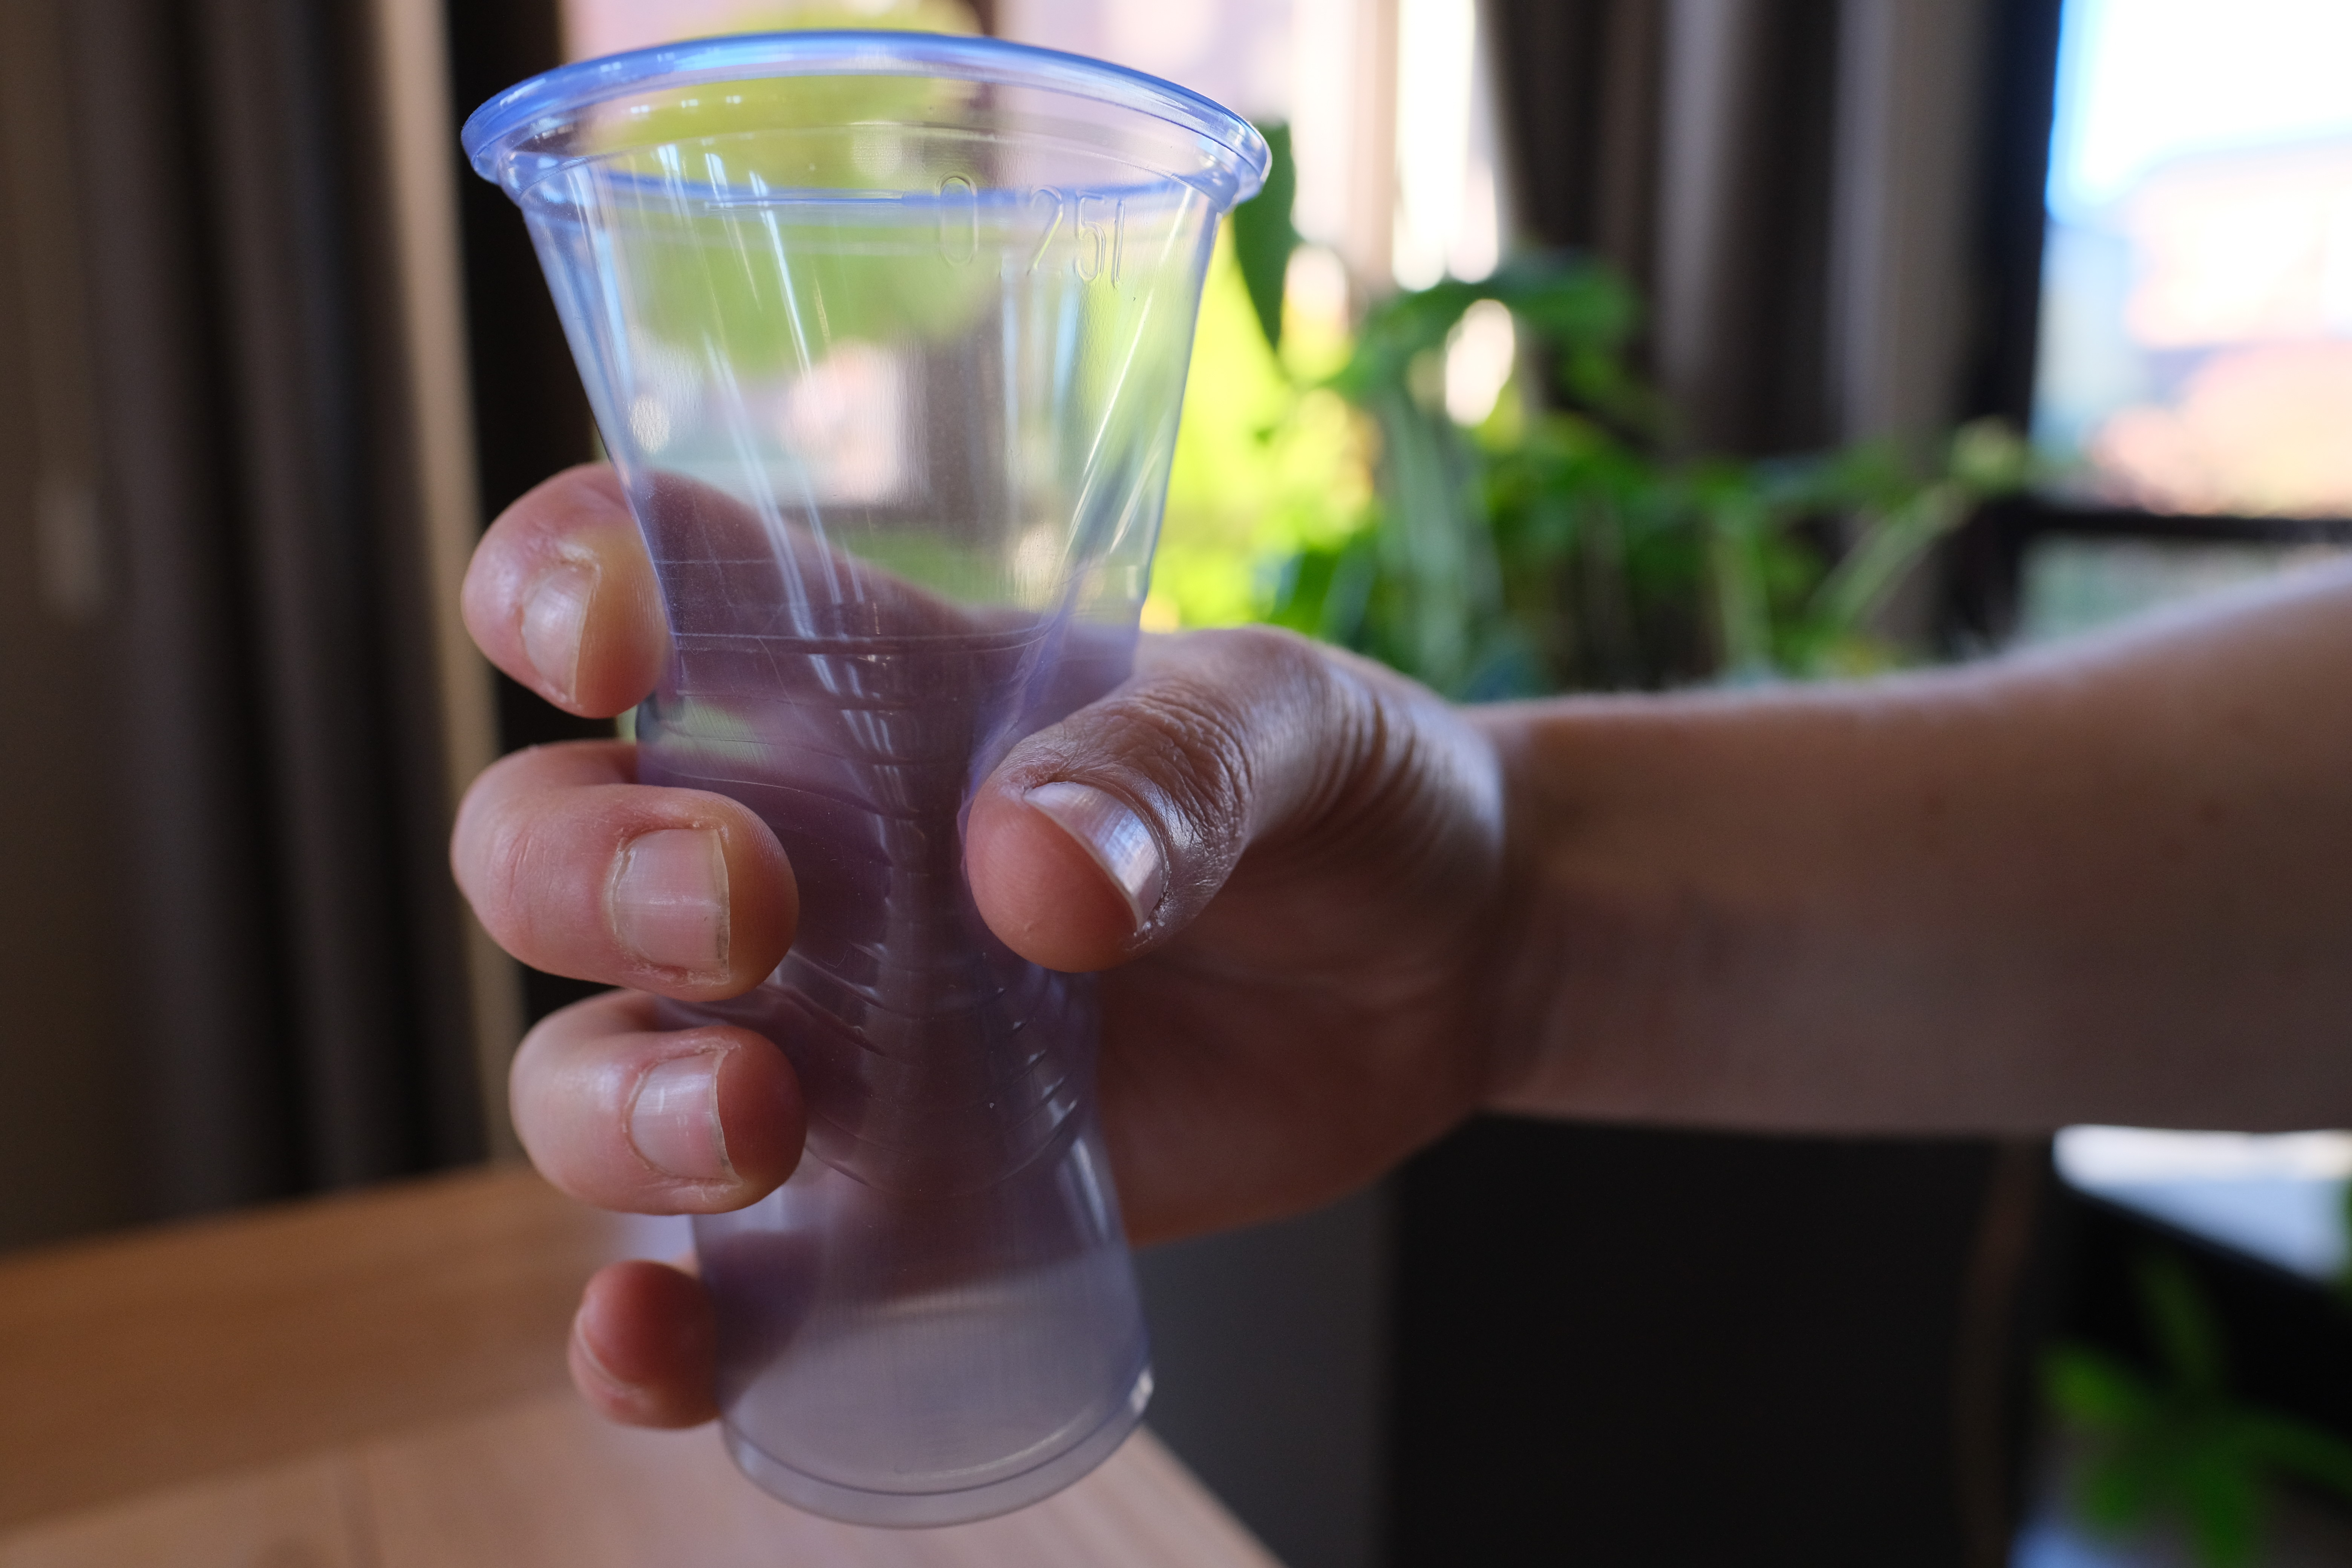
\includegraphics[keepaspectratio, width=\textwidth]{figures/fig_cup.JPG}
        \caption{}
        \label{fig:force_closure_deform_object_cup}
    \end{subfigure}

    \caption[Force closure examples.]{Force closure on a rigid glass (a) and a deformable, plastic cup (b). The deformations of the plastic cup need to be taken into account when calculating a grasping pose.}
    \label{fig:force_closure_deform_object}
\end{figure}

\subsection{Deformable objects: definition, categorization, tasks and solutions}
% Vervormbare objecten: wat zijn ze, categorisatie, welke taken en welke oude pipelines bestaan er
A deformable object is an object whose shape changes when being subject to an external force. This deformation can be temporary and reversible (\textit{elastic}), permanent (\textit{plastic}) or a combination of both (\textit{elasto-plastic}). Deformable objects are found in industrial settings, agriculture and household items. A common categorization \autocite{Saadat2002,Jimenez2012} is based on the geometry of the object: how many dimensions are significantly larger than the other dimensions. The rationale for this categorization is given by small dimensions of the object having a negligible impact on the deformable properties. A canonical example where this property is applied is found in the sheet metal bending industry: the thickness of metal sheets is neglected when computing the required manipulations for bending \autocite{Duflou2005}. A consequence of this categorization is that 3D objects can be considered as 2D deformable objects. For example, both a hollow rubber ball and plush ball can be considered 3D deformable objects based on their dimensionality. However, when considering the dimensions that only impacts the deformable properties, a hollow ball is 2D deformable object as the thickness can be neglected for manipulation. 
\keyWithTitle{Deformable objects}{A deformable object is an object whose shape changes on interaction and can be categorized based on the number of dimensions negligible for manipulation planning.}
In its simplest setting, the deformable object is one dimensional: ropes, strings, cables, threads and catheters, among others. Some of these examples are shown in \cref{fig:dlo_examples}. These objects are also known as deformable linear objects. The term \textit{linear} refers to one dimension being dominant over the other two dimensions. Common tasks for deformable linear objects involve grasping and manipulating ropes, for example, knot tying. Early motor control architectures for solving tasks regarding deformable linear objects used either an open-loop approach or simple visual servoing to execute the motion. An early work clearly demonstrating modular control pipelines is the project of~\citeauthor{Inaba1987} in~\citeyear{Inaba1987}. Their method employs visual servoing for manipulating a rope into a ring and then tying the rope. 
Their perception module uses stereo images to detect the rope and the ring. The planning module is hard-coded to iterate through a set of predefined steps while using the detected centre of the ring and 3D coordinates of the endpoints of the rope from the perception module. An inverse kinematics module provides a target trajectory to the low-level controller. Similar modular pipelines can be found in \autocite{Remde1999} for grasping a rope and in \autocite{Saha2007} where knots are tied with needles using probabilistic trajectories of the rope from a simulated model. Incorporating motion primitives, i.e.\ a predefined set of motor actions corresponding to high-level actions, in the planning module is used in \autocite{Yamakawa2008, Vinh2012} to tie knots in a rope.

\begin{figure}[htbp!]
    \centering
    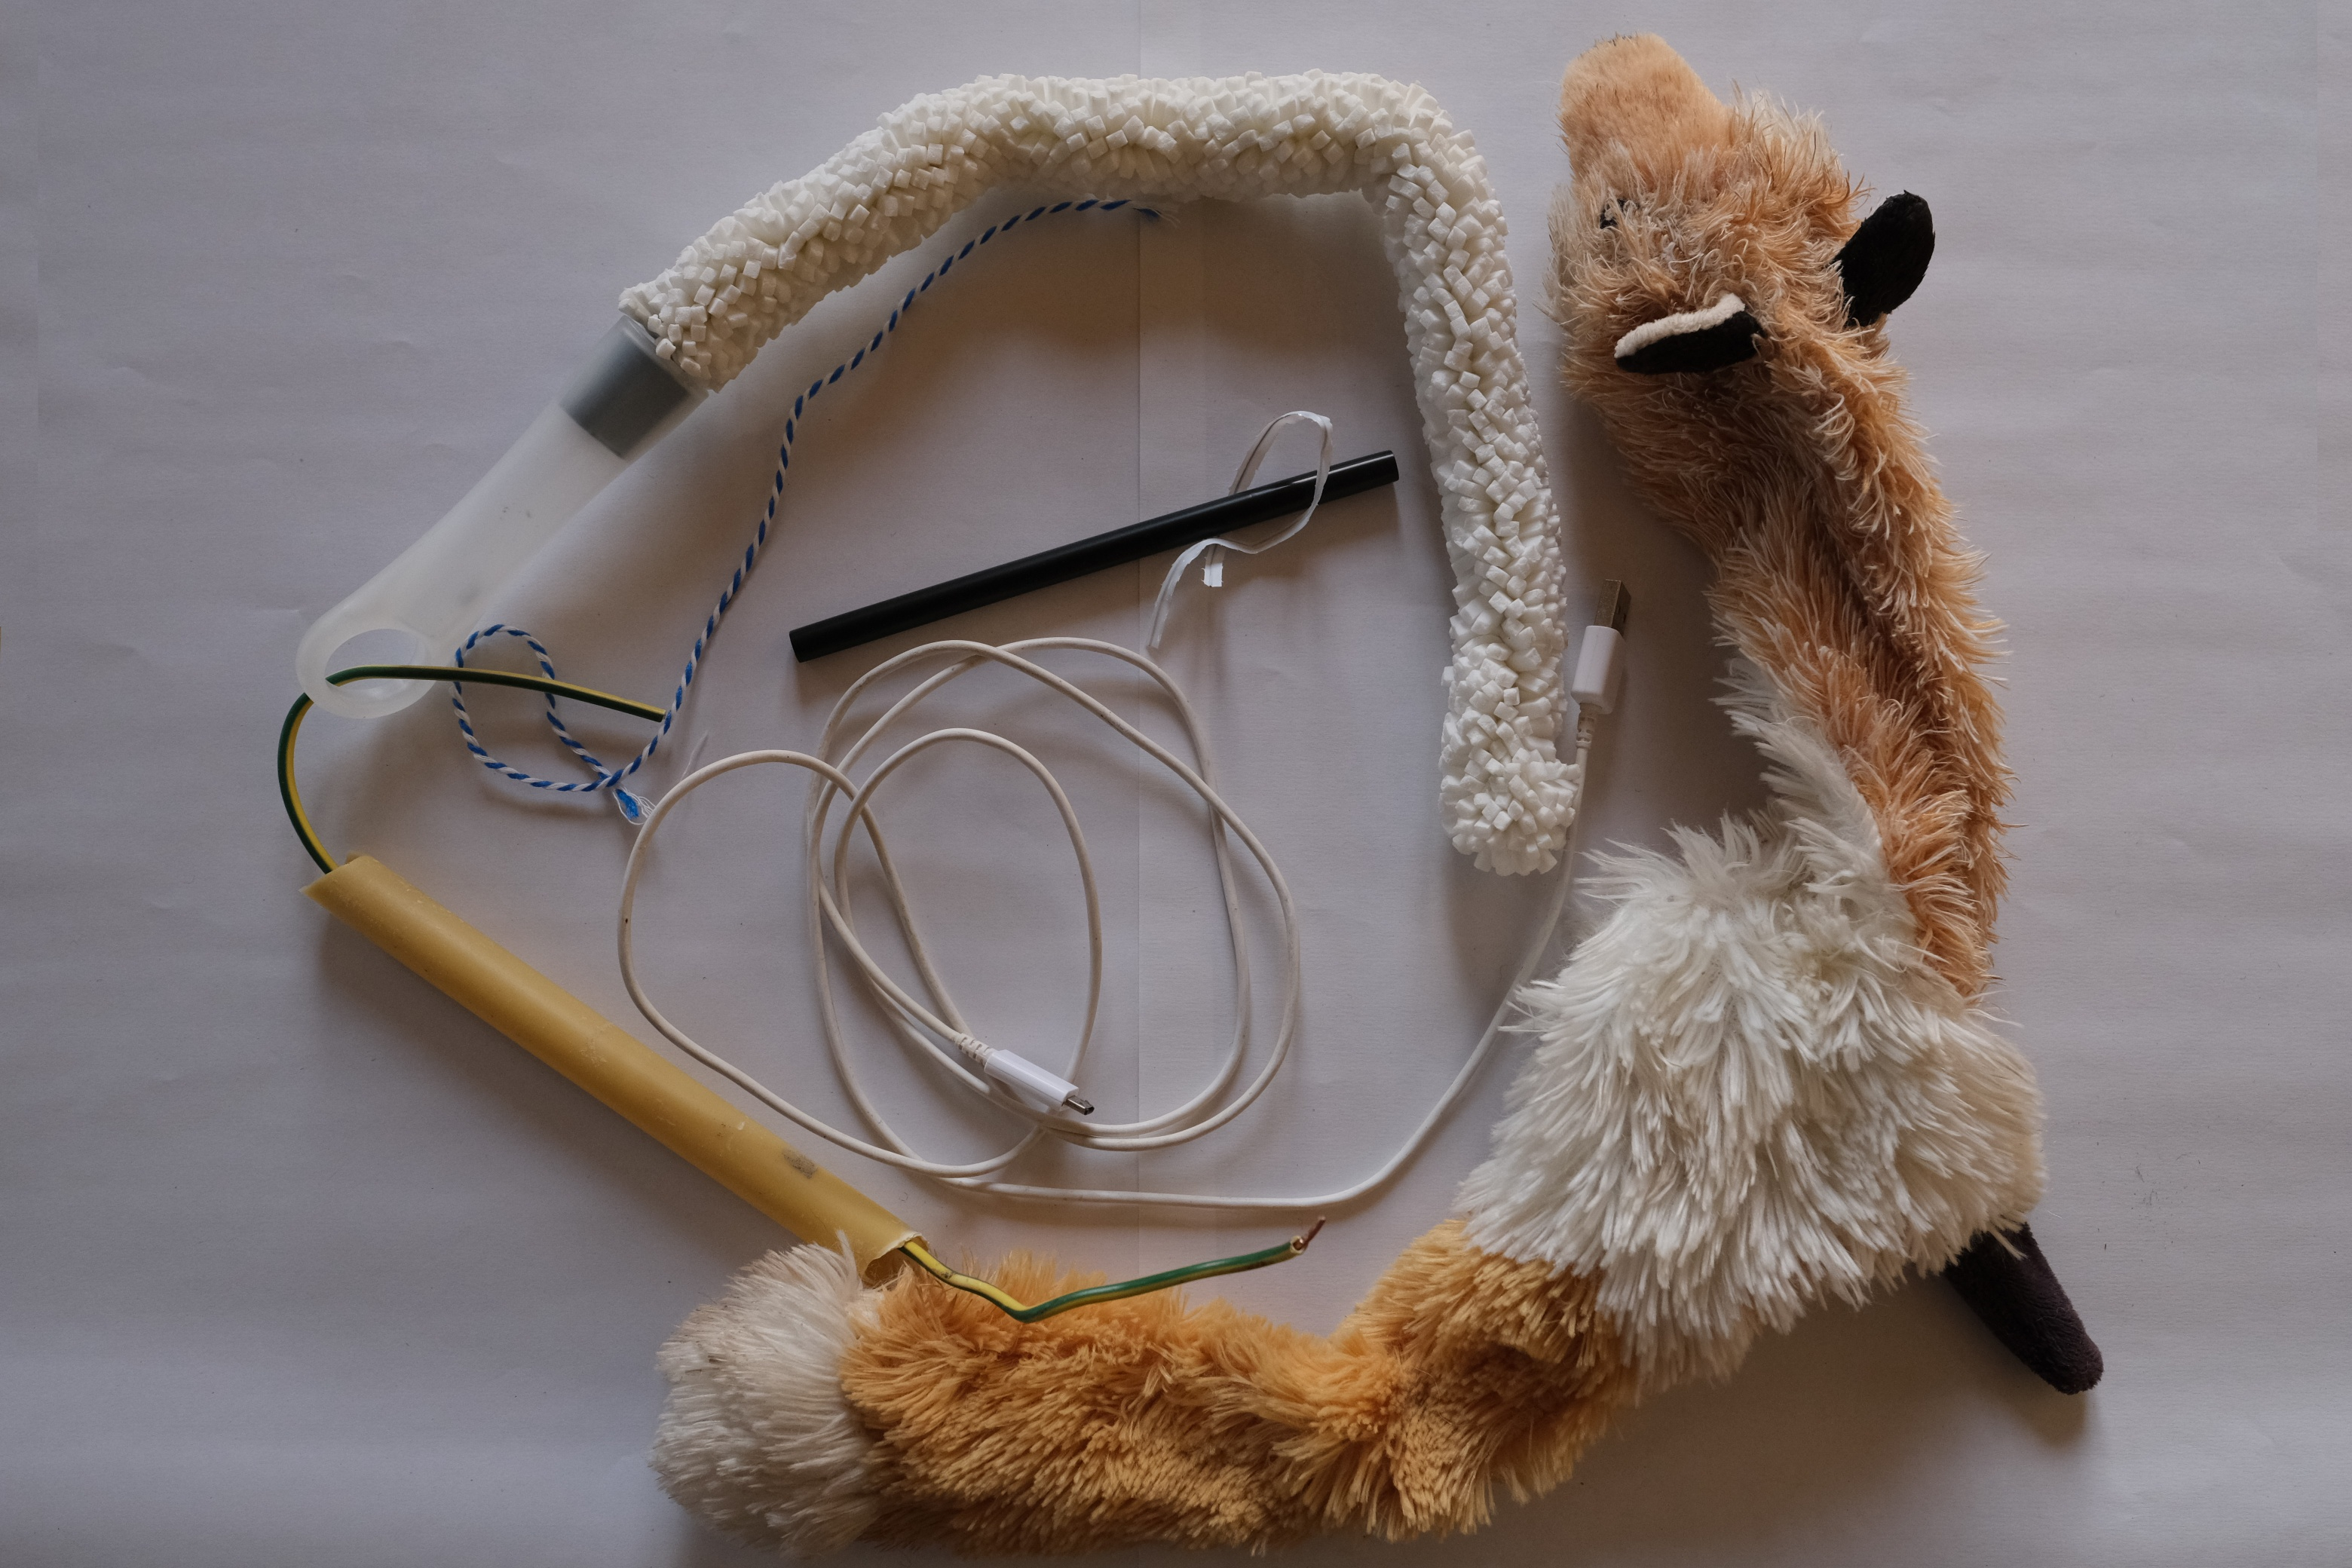
\includegraphics[keepaspectratio,width=\textwidth]{figures/fig_dlos.JPG}
    \caption[Real-life examples of deformable linear objects.]{Examples of deformable linear objects and an application of putting an electrical wire into a rigid pipe.}
    \label{fig:dlo_examples}
\end{figure}

% 2D objects klassieke pipelines
Deformable \textit{linear} objects become deformable \textit{planar} objects when two dimensions are significantly larger than the third dimension. 
In this case, the planning module can disregard the thickness of the material for manipulation. Canonical examples are given in \cref{fig:planar_deform_objects_examples} and contain objects such as clothing, thin-shelled objects like plastic bottles, fabric, paper, and plastic bags, deformable sheets, cards and foam materials. A classic example of paper folding is robotic origami, in which a robot has to sculpt a piece of paper into the desired shape by folding. This problem was tackled with an open-loop control architecture in \autocite{Balkcom2008} to produce a folded hat. \Textcite{Elbrechter2012} takes this a step further by using vision, simulation and fiducial markers on the paper to grasp and fold a paper with a five-fingered end-effector. Related to origami is carton folding and metal sheet bending. Typical control strategies \autocite{Liang1999,Liu2003,Aomura2002} consist of finding the correct locations and sequence of bending operations by modelling the object as a collection of panes articulated through hinge joints. Robotic manipulation of bags has been less studied due to the complexity of modelling and manipulating bags. To circumvent this complexity, dedicated hardware has been researched for grasping \autocite{Kazerooni2005} and unloading \autocite{Kirchheim2008} sacks. A general-purpose two-fingered robotic gripper is used in \autocite{Klingbeil2011} to grasp objects from a table, search the barcode and drop the object into a bag. The planner uses 3D points clouds of depth images taken by a camera. However, they assume the bag is already open for insertion and do not consider any possible deformations caused by touching or dropping an item into the bag.

In the context of this research, it is of interest to note that garments satisfy the same geometrical property of having one negligible dimension as objects such as paper and plastic bottles. However, the main characteristic distinguishing cloth is the compression strength: compared to other two-dimensional deformable objects, cloth does not possess any significant compression strength. Given that the current work deals with manipulations of clothing items, we dedicate \cref{sec:lit_cloth_folding_pipelines} to elaborate on cloth manipulation pipelines.

\begin{figure}[htbp!]
    \centering
    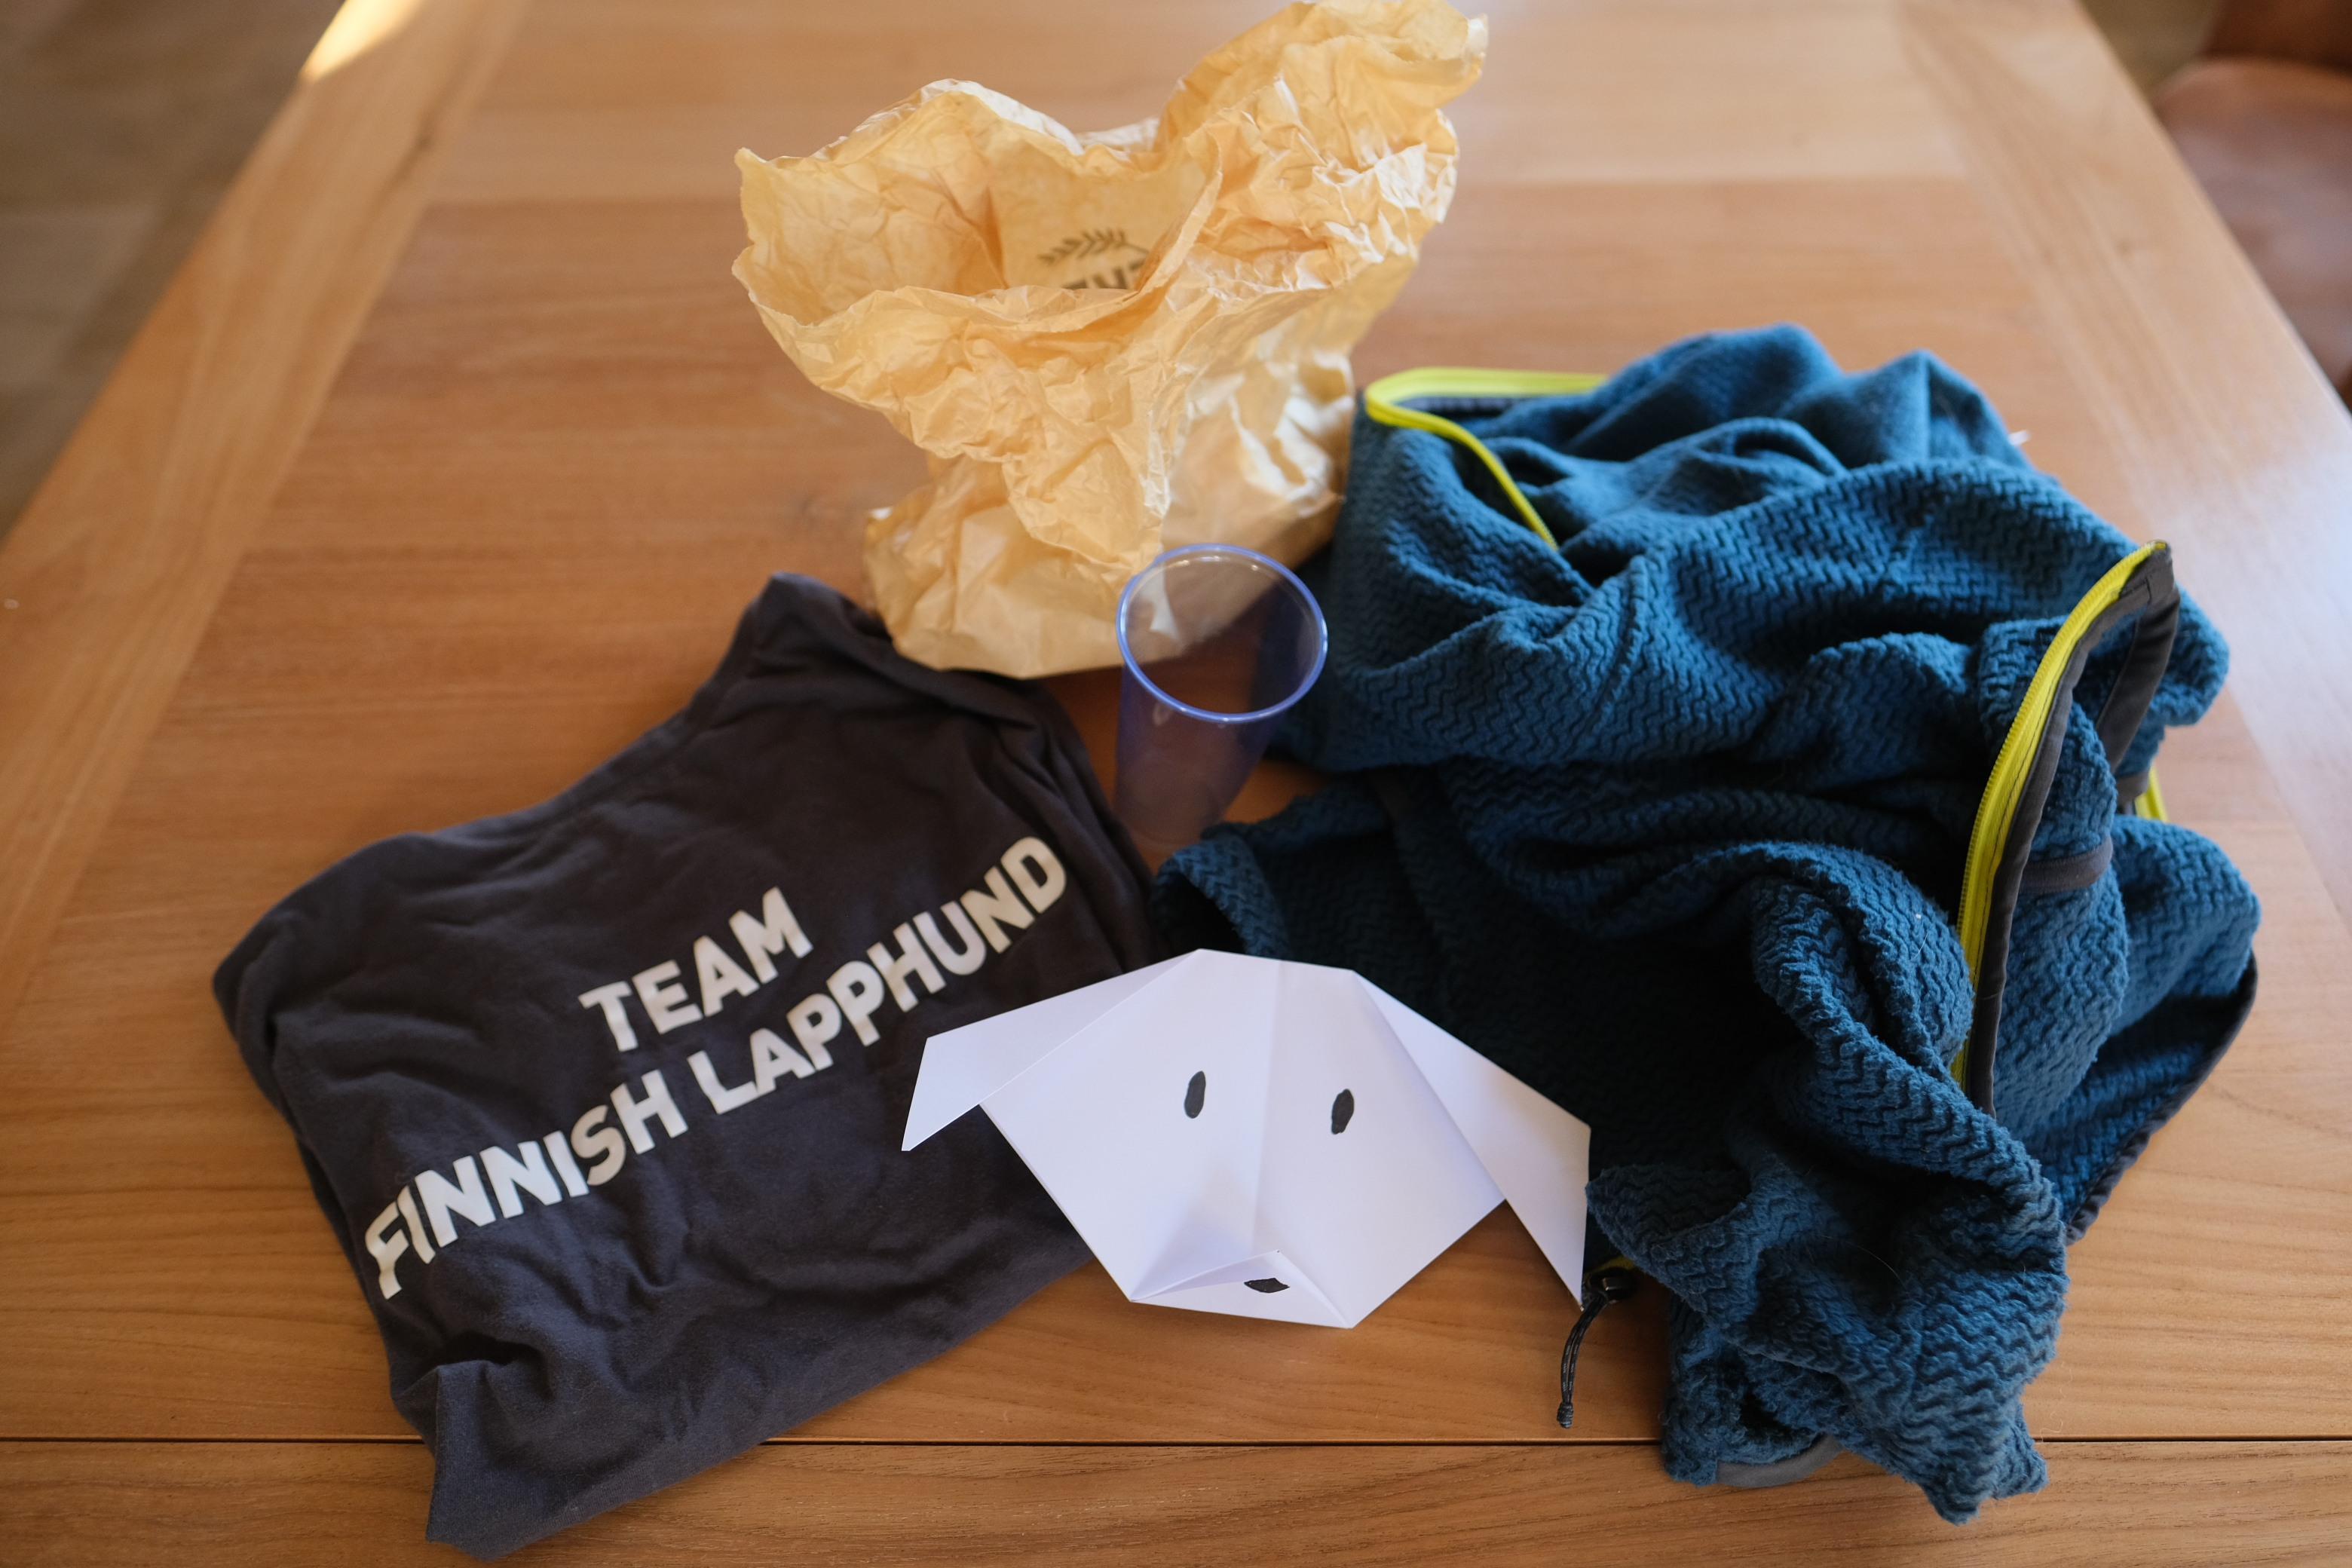
\includegraphics[keepaspectratio,width=\textwidth]{figures/fig_2d_deformables_ex.JPG}
    \caption[Examples of 2D deformable objects]{Examples of 2D deformable objects: origami, paper bag, shirt, jumper and a cup.}
    \label{fig:planar_deform_objects_examples}
\end{figure}

% 3D objects klassieke pipelines
The final category of deformable objects is \textit{volumetric deformable objects} whose deformations across all dimensions of the object are of relevance. Some examples are shown in \cref{fig:volumetric_deform_objects_examples}: objects such as food, plush toys and sponges. In the case of food products, deformations can be caused by both grasping and processing operations such as slicing. In general, 3D deformable objects are the least researched type of deformable objects \autocite{Sanchez2018}. An exception to this is soft tissue, which is important for medical application. We refer the reader to the review paper by \textcite{Taylor2016} for an overview of medical robots in surgery applications. An overview of robotic manipulation of food products is given in \textcite{Chua2003}.

\begin{figure}[htbp!]
    \centering
    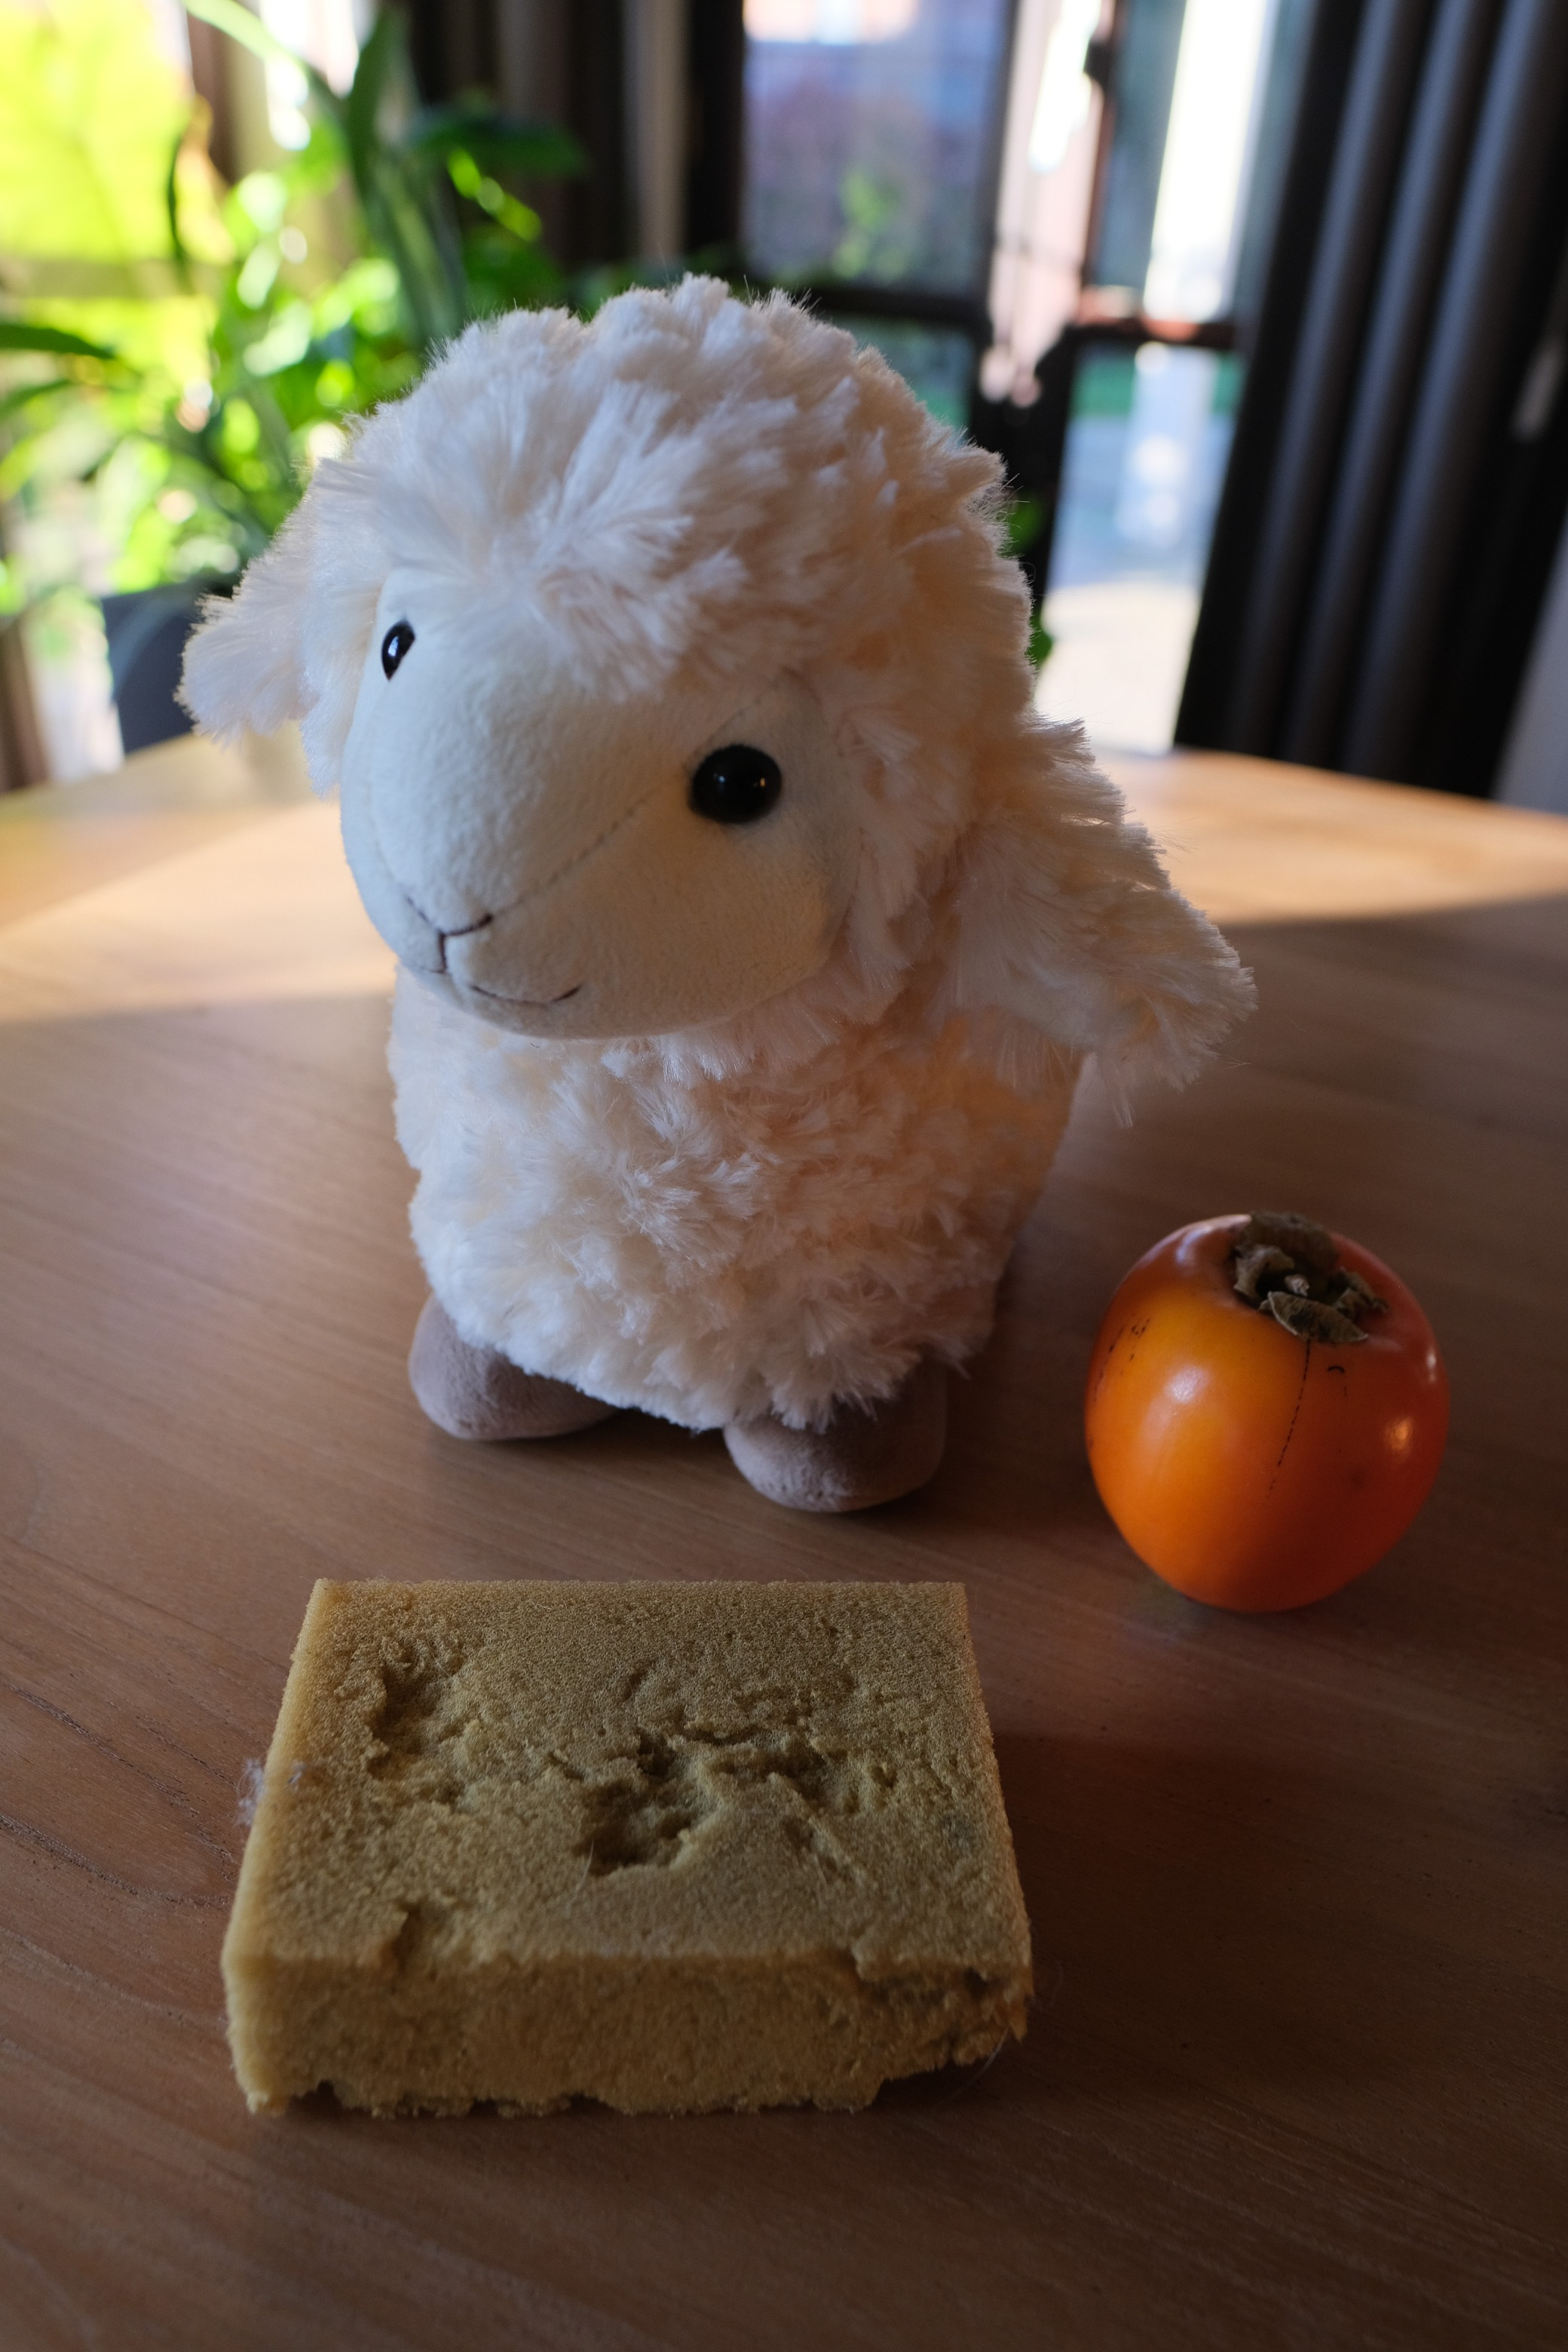
\includegraphics[keepaspectratio,width=\textwidth]{figures/fig_3d_deformables_ex.JPG}
    \caption[Solid deformable objects]{Examples of volumetric deformable objects: sponge, fruit and plush toy}
    \label{fig:volumetric_deform_objects_examples}
\end{figure}

\section{Learning-based approaches to robotic manipulation} \label{sec:lit_learning}

Machine learning, a domain of artificial intelligence, is the study of algorithms that give computers the ability to learn from and make predictions based on data. Learning provides a viable alternative for robotics as it gives a way to deal with the inherent systematic as well as random errors in robotic systems and variability in unstructured environments. This is because in learning, you optimize for the grasping task, which implicitly adapts the behaviour to imperfections in the system such as inaccurate sensor readings.

In this section, we provide a short review on the fundamentals of relevant machine learning techniques. In order to provide background on \acrfull{DRL}, i.e. the method used in this thesis, we describe supervised learning methods (\cref{subsec:lit_sl}), deep neural networks (\cref{subsec:lit_dnn}) and reinforcement learning (\cref{subsec:lit_rl}). We discuss their relevant applications in robotic manipulation with a focus on manipulation of deformable objects. This section aims to provide an understanding on these domains, based on required essentials. For a comprehensive view on the machine learning field, the reader is referred to~\autocite{Friedman2001} and~\autocite{Bishop2006}.

\subsection{Supervised learning} \label{subsec:lit_sl}

% inspiratie: boek gabriel, matthias, jim. ML course NG, DL book ch5

Supervised learning is a machine learning paradigm where there is a set of \textit{input} variables that exert influence over other \textit{output} variables. For example \dots. More formally, we can denote the input data as a set X consisting of vector x in X. In the machine learning domain, this set of predictor variables is often called \textit{features}. The set Y contains the output variables y in Y. Concatening tuples of (xi, yi) leads to a dataset which can be used for learning. 

STRUCTUUR:
	Definition: dataset, models , OF optimization, grad descent, splits 
	Application in robotic learning:
		perception modules of modular pipelines
		imitation learning: survey argall 
		direct learning: dexnet, google levine paper 
		(! focus on cloth applications)


The learning happens in the 'model'. Can be many things: decision trees, linear models, ANNs. 
Central idea is to change parameters of the model such that the outputs of the model matches the outputs of dataset, given the inputs. 
grad descent. 


\subsection{Unsupervised learning}
Definition
Relevance:
	 dimensionality reduction: PCA, T-sne, UMAP 
	 clustering 
Application in learning (very short): visualization of embeddings, separation of cloth, ... 


\subsection{Deep neural networks} \label{subsec:lit_dnn}
Structure: 
	- Motivation: representation matters
	- ANN, MLP basics: neurons, activations, nonlinearities, layers, feedforward, 
	- optimization: backpropagation 
	- CNNS
	- Increasingly abstract representation through deep layers 
	- Applications in robotics:
		perceptual module in pipelines
		dexnet, google levine paper
		cfr review deep learning in robotics 

Comprehensive review on~\acrshortpl{DNN}, see the textbook of~\textcite{Goodfellow2016}.

\subsection{Reinforcement learning} \label{subsec:lit_rl}
contrast to SL 
why relevant for robotics
MDP formalisatie
from bellman equation to q-learning 
RL loop and elements: state representation, reward function. 
RL architectures and categorization: value based, policy methods, actor critics 
Applications in robotic manipulation and cloth 

Reinforcement Learning is an eminent approach for learning control policies with no user intervention. A complete review of RL is outside the scope of this thesis. Therefore, we refer the reader to the standard textbook of~\textcite{Sutton2018}.

\section{Datasets for robotic learning} \label{sec:lit_datasets}
Motivatie:
	Link met SL
	Link met RL, offline RL 

Kan simulatie of echte data zijn. 

Relevante werken:
	DexNet, 

\section{Simulation environments to accelerate learning} \label{sec:lit_simulation}

Motivatie voor simulatie: dure, trage robot tijd 
Componenten: physics engine, robot simulatie, link naar fysische platform.

\subsection{Cloth simulation methods} \label{subsec:lit_cloth_sim}
%Zie ook "Robotic manipulation and sensing of deformable objects in domestic and industrial applications: a survey" p4 voor overzicht om te introduceren maar focus op particle based methods.

Wat maakt cloth simulatie moeilijk. 
Aanpakken tot cloth simulatie (kort de categorisatie)
Particle based method. 
Integrators. 
Ander werk dat gebruik maakt van cloth simulatie voor robotic maniulation.

\subsection{Transferring simulation results to the real world}  \label{sec:lit_sim2real}
sim2real problem uitleggen.
Verschillende aanpakken uitleggen: Meta learning, simulatoin randomization, system identifitcation, domain adaptation
literatuur bespreken. 

\section{Reward learning}  \label{sec:lit_reward_learning}
General introduction 
Motivatie: Reward hacking, impossible to capture all ingredients
Literatuur: 
	IRL 
	Reward learning 

\section{State perception through instrumentation} \label{sec:lit_instrumentation}
Motivatie.
Definitie.

literatuur:


\end{document}